\documentclass[numbers=noenddot,12pt,a4paper]{scrartcl}
\usepackage[greek,ngerman]{babel}
\usepackage[T1]{fontenc}
\usepackage[utf8]{inputenc}
\usepackage{ifoddpage}
\usepackage{libertine}
\usepackage{ziffer}
\usepackage{graphicx}
\usepackage{units}
\usepackage[infoshow]{tabularx}
\usepackage{amsmath}
\usepackage{fancyhdr}
\usepackage{amssymb}
\usepackage{wrapfig}
\usepackage{esint}
\usepackage{float}
\usepackage{wrapfig}
\usepackage[font=small]{caption}
\usepackage{subcaption}
\usepackage{lscape}
\usepackage{hyperref}

\renewcommand{\thefigure}{Abb. \arabic{figure}}

\captionsetup[wrapfigure]{name=}
\captionsetup[figure]{name=}
\newcommand{\degree}{^\circ}
\newcommand{\diff}{\textnormal{d}}
\newcommand{\tenpo}[1]{\cdot 10^{#1}}
\newcommand{\greek}[1]{\greektext#1\latintext}
\newcommand{\ix}[1]{_\text{#1}}
\newcommand{\imag}{\mathbf{i}}
\newcommand{\tilt}[1]{\textit{#1}}
\newcommand{\grad}[1]{\textit{grad}\left(#1\right)}
\newcommand{\divergenz}[1]{\textit{div}\left(#1\right)}
\newcommand{\euler}{\mathnormal{e}}
\newcommand{\fett}[1]{\textbf{#1}}
\renewcommand{\headrulewidth}{0.1pt}
\renewcommand{\footrulewidth}{0.1pt}
\newcommand{\name}{\text{Alexander Jankowski}} 

\title{Protokoll: Positronen und Koinzidenzmessung}
\author{Alexander Jankowski, Philipp Hacker}
\date{\today}
\pagestyle{fancy}
\fancyhead[C]{\thepage}
\fancyhead[R]{\name}
\fancyfoot[C]{\thepage}
\fancyhead[L]{Abschnitt \thesection}
\begin{document}
	\maketitle
	\begin{center}
		Betreuer: Gerrit Marx \\ 
		Versuchsdatum: 21.10.2015\\ 
		\begin{table}[h]
			\centering
			Note: 
			\begin{tabularx}{1.5cm}{|X|}
				\hline \\ \\
				\hline
			\end{tabularx}
		\end{table}
	\end{center}
	\vspace*{\fill}
	\tableofcontents
	\vfill
	\newpage

\section{Motivation}
In gewöhnlicher Materie sind Positronen in der Regel keine stabilen Teilchen, da diese mit den vorhandenen Elektronen reagieren und durch Paarvernichtung unter Abgabe von elektromagnetischer Strahlung zerfallen. Um diesen Zerfall zuverlässig untersuchen zu können, ist es notwendig die gemessene Ereignisse zuverlässig dem richtigen Ursprung zuzuordnen. Dafür wird in diesem Versuch ein Aufbau studiert, welcher eine koinzidente Messung zweier Zeitnaher Ereignisse zulässt, um diese dem selben Zerfall zuzuordnen.
\newpage

\section{Physikalische Grundlagen}

	\subsection{Positron}
		
		Das Positron $e^+$ ist ein Elementarteilchen und gehört zu den Leptonen. Es ist das Antiteilchen zum Elektron, hat eine positive Elementarladung $+e$ und besitzt eine Ruheenergie gleich der eines Elektrons von $E_0 = 511\,\mathrm{keV}$. In der Natur entstehen Positronen durch den Zerfall von positiven Myonen oder durch $\beta^+$-Zerfall von radioaktiven Kernen. Positronen haben in gewöhnlicher Materie eine kurze Lebensdauer, da sie durch den Prozess der Paarvernichtung mit Elektronen unter Abgabe von Strahlung annihiliert werden.

		\subsubsection{Zerfall von $^{22}\textrm{Na}$}
	
			Positronen entstehen unter anderem bei dem $\beta^+$-Zerfall von $^{22}\textrm{Na}$-Kernen mit einer Halbwertszeit von $2,6$ Jahren.
	
			\begin{equation}
				^{22}\textrm{Na} \rightarrow {}^{22}\textrm{Ne}^* + e^+ + \nu_e
			\end{equation}
	
			Die weiteren Produkte des Zerfalls sind ein Neon Atom ${}^{22}\textrm{Ne}^*$, welches sich in einem angeregtem Kernzustand befindet, und einem Elektronen Neutrino $\nu_e$. Der Neon Kern wechselt anschließend über die Abgabe eines $\gamma$-Photons mit einer Energie von $E_\gamma = 1\,275\,\mathrm{keV}$ in den Grundzustand. Dieses Photon wird für diesen Versuch genutzt um einen definiertes Startsignal für die Messung eines Ereignisses festzulegen.
			
			\begin{equation}
				{}^{22}\textrm{Ne}^* \rightarrow {}^{22}\textrm{Ne} + \gamma
			\end{equation}
			Die Lebensdauer des angeregten Neon Kern beträgt nur $3,7\,\mathrm{ps}$ und kann daher im Vergleich zum Zerfall des Natrium Kerns als instantan angesehen werden. 
	
		
		\begin{figure}[!h]
			\centering
			\label{abb:zerfall}
			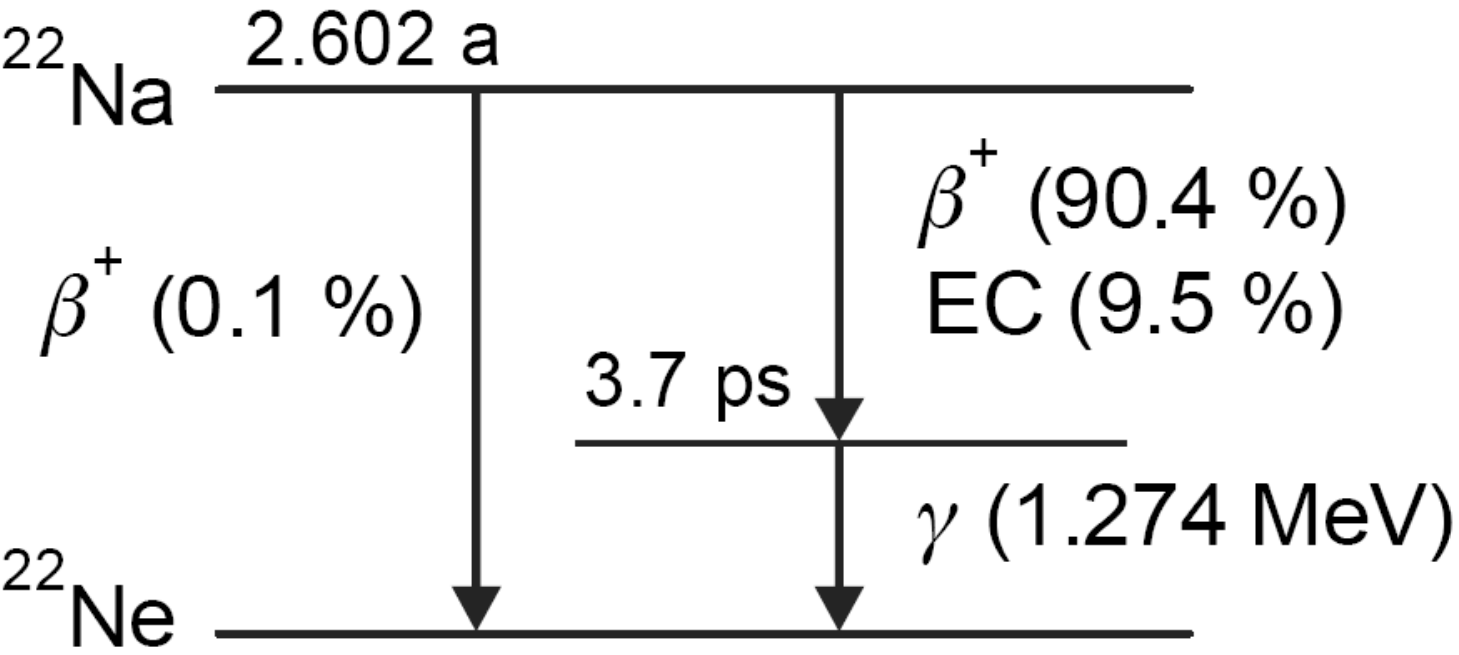
\includegraphics[width=0.5\columnwidth]{pics/termschema}
			\caption{Niveau Darstellung des $\beta^+$ Zerfalls von ${}^{22}\textrm{Na}$. Der rechte Zerfallsweg ist hierbei der dominante. In diesem wird ein zusätzliches $\gamma$-Photon mit einer Energie von $1,274\,\mathrm{MeV}$ frei.}
		\end{figure}
	
		\subsubsection{Paarvernichtung, Positronium und Lebenszeiten}
	
			Trifft ein Positronium $e^+$ auf ein Elektron $e^-$ so kommt es zur Paarvernichtung. Dabei löschen sich die Teilchen gegenseitig aus und ihre Energie wird in zwei $\gamma$-Photonen überführt, welche in sich einem Winkel von ca. $180^\circ$ zueinander ausbreiten.
	
			\begin{equation}
				e^+ + e^- = 2 \gamma
			\end{equation}
	
			Die Photonen haben jeweils eine Energie, die der Ruheenergie des Positrons bzw. Elektrons entspricht.
			
			\begin{equation}
				E_\gamma = E_0 = m_e c^2 = 511\,\mathrm{keV}
			\end{equation}
	
			Das durch den $\beta^+$-Zerfall entstandene Positron verfügt über eine hohe kinetische Energie. In Materie wird das Positron Coulombstöße mit den Kernen und Elektronen ausführen. Dabei gibt es kinetische Energie ab, bis es genug abgegeben hat, um eventuell einen bindenden Zustand mit einem Elektron einzugehen. Dieses Teilchen aus einem gebundenen Elektron und Positron wird Poitronium genannt. Diese Bindung ist metastabil und endet ebenfalls in der Anihilierung der beiden Bindungspartner, jedoch mit einer höheren Lebenszeit als der spontane Fall.
	
			Weiterhin wird beim Positronium je nach Spinkonfiguration zwischen zwei verschiedenen Grundzuständen mit verschiedenen Lebenszeiten unterschieden. Im Fall von antiparallelen Spin spricht man vom Para-Positronium mit einer Lebenszeit von $t_\mathrm{para} = 1,24\cdot10^{-10}\,\mathrm{s}$ und im Falle von parallelen Spins vom Ortho-Positronium mit einer Lebenszeit von $t_\mathrm{ortho} = 1,42\cdot10^{-7}\,\mathrm{s}$.
	
		\subsection{Koinzidenzmessung}
			
			Bei einer Koinzidenzmessung werden zwei zusammenhängende Ereignisse in einer kurzen Zeitspanne gemessen. Der Zeitraum für die Messung eines indiviuellen Ereignisses beträgt hierbei nur Pico- bis Nanosekunden. Um die Unterscheidung für verschiedenen gemessene Ereignisse zu gewährleisten ist eine schnelle und empfindliche Elektronik erforderlich, welche für Messungen in einem kurzen Zeitraum ausgelegt ist. Um eine solche Messung durchzuführen ist es notwendig einen gut definierten Startzeitpunkt zu setzten. Diesen liefert das hoch energetische $\gamma$-Photon ($1,274\,\mathrm{MeV}$), welches idealerweise zeitgleich mit dem Positron beim Kernzerfall von ${}^{22}\mathrm{Na}$ entsteht. Dieses kann durch einen Szintilationszähler detektiert werden und starten einen Messvorgang. Diese Szintillationsschirme haben eine sehr geringe Todzeit zwischen zwei Ereignissen und können mit Hilfe der Elektronik die eingehenden Photonen energieaufgelöst darstellen.\\
			Die Ereignisse welches nach dem Start der Messung detektiert werden sollen, sind die beiden $511\,\mathrm{keV}$-Photonen, welche im Idealfall von zwei einander entgegen gerichteten Szintillationsschirmen detektiert werden. 
			
\newpage

\section{Aufbau und Durchführung}

	\subsection{Geräteliste}
		
		Der Versuch besteht zum einem aus der radioaktiven ${}^22\mathrm{Na}$-Präparat, welches unter einer Abschirmung zwischen zwei Detektoren angebracht ist, so dass diese jeweils einen möglichst großen Raumwinkel, vom Präparat ausgehend, abdecken, und zum anderen aus der Messelektronik zur Verarbeitung des Detektorsignals. In diesem Versuch wird das {}"Positron Lifetime System Setup{}" der Firma Ametek verwendet. Wichtige Bestandteile sind
		\begin{itemize}
			\item zwei 265A Scintillationsdetektoren,
			\item zwei 556 High Voltage Power Supplies,
			\item zwei 583B CF Discriminator Module,
			\item ein 414A Fast Coincidence Modul,
			\item zwei DB463 Delay Module,
			\item ein 567 TAC Modul,
			\item ein 113 Preamplifier,
			\item ein 575A Amplifier Modul,
			\item ein Multi Channel Analyzer (MCA).
		\end{itemize}
		Weiterhin wird ein Oszilloskop zur Analyse des Signals und ein Computer zur Datenaufnahme verwendet. Die Elektronik wird für die einzelnen Kalibrierungsschritte und die Messung verschieden verkabelt.
		

	\subsection{Kalibrierung}
		
		Im ersten Schritt der Kalibrierung wird das Anodensignal beider Detektoren auf dem Oszilloskop überprüft und an den 556 Powersupplies auf eine Signalstärke von $1\,\mathrm{V}$ eingestellt. Für die weiteren Schritte wird der Dynodenausgang der Detektoren mit Hilfe des 113 Vorverstärkers und des 575A Verstärkers auf den Eingang des MCAs gelegt.\\
		Im nächsten Schritt werden die "constant fraction" Diskriminatoren 583B (CFD) auf den Start- bzw. den Stoppuls kalibriert. Das Signal eines Detektors wird auf den Eingang des CFDs gelegt. Wird ein bestimmter Schwellwert überschritten, so produziert der CFD ein logisches Signal mit definierter Pulsdauer. Um zu verhindern, dass zeitgleiche Signale verschiedene Ergebnisse produzieren, sind die Eingänge vom CFD so eingestellt (Verschiebung, Stauchung), dass alle Ereignisse gleich aufgelöst werden. Der Ausgang des CFDs wird nun an den 567 {}"time to analog conveter{}" (TAC) Starteingang angeschlossen und dann über den {}"Valid Start Out{}" Ausgang auf das Gate des MCAs gelegt. In diesem Aufbau kann durch eine Messung die Abschnittskanten für das Start- bzw. das Stoppsignal kalibriert werden.
		
		Bevor eine Messung zur Bestimmung des Zerfallskonstanten für Positronen durchgeführt werden können, muss den Kanälen im Detektor eine entsprechende Zeit zugeordnet werden. Dafür wird die Elektronik wie in Abb. aufgebaut und eine zeitaufgelöste Messung gestartet. Am {}"DB463B Delay{}" Gerät werden im Laufe der Messung verschiedene Zeitdelays ($0 - 32\,\mathrm{ns}$) eingestellt um ein Spektrum zu erzeugen an welchem die Zeit pro Kanal für weitere Aufnahmen kalibriert werden kann.
		\\
		Die eigentliche Messung findet im Aufbau nach Abb.\ref{abb:aufbau} statt. Bei dieser Verschaltung wird bei der Detektierung eines Startphotons eine Messung zur Detektierung des Stoppphotons gestartet und bei einem positiven Ereignis wird ein Signal vom MCA an den Computer geschickt, wo die Messsoftware ein zeitaufgelöstes Spektrum aufnimmt. Die Messung in diesem Aufbau dauert ca. 12 Stunden.
	    
	    		\begin{figure}[!h]
	    			\centering
	    			\label{abb:aufbau}
	    			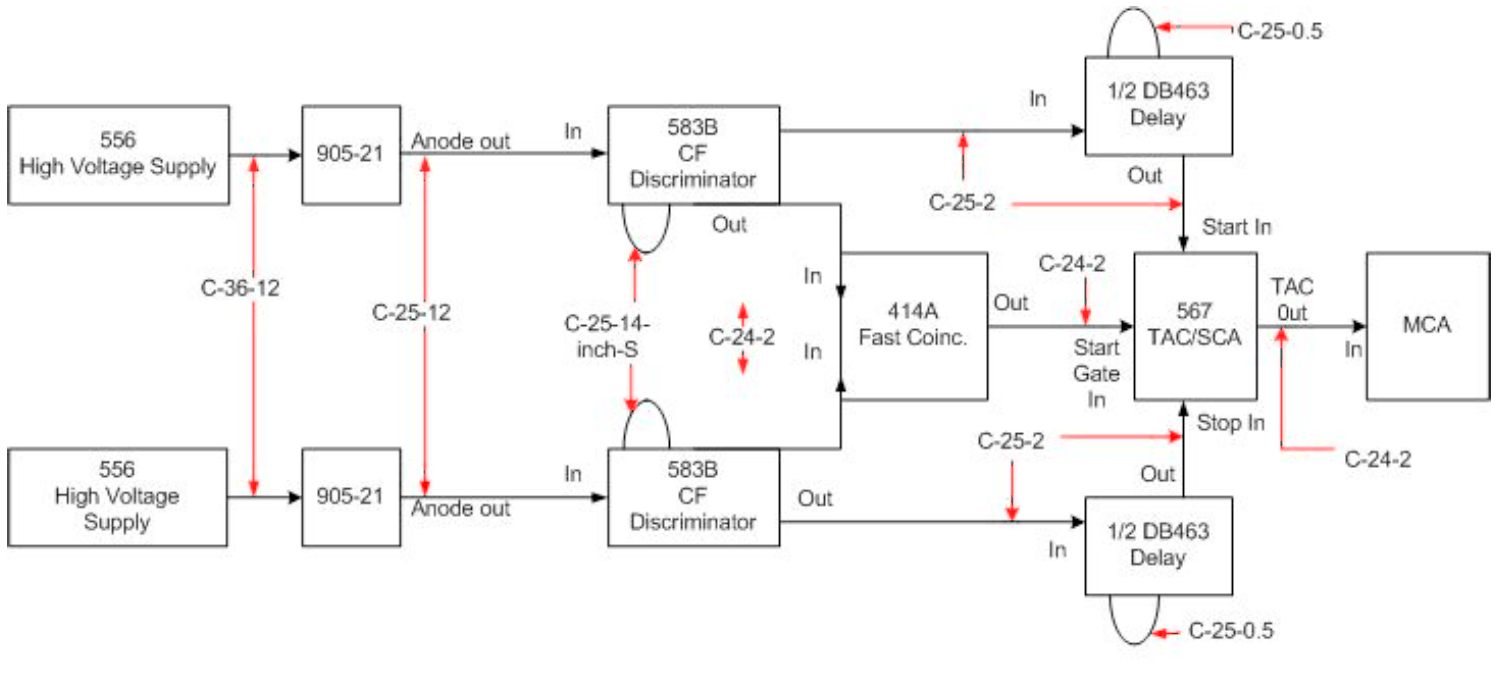
\includegraphics[width=1\columnwidth]{pics/aufbau}
	    			\caption{Schaltschema für die Messung der Lebenszeit der Positronen. Der MCA ist and einem Computer zur Datenaufnahme angeschlossen.}
	    		\end{figure}
	    
\newpage

\section{Auswertung}
	
	\subsection{Zeitkalibrierung}

		Aus der Kalibrierungsmessung (vgl. Abb.\eqref{abb:Zeitkal}) werden zu den entsprechenden Zeitschritten die Maxima des Signals ausgelesen und durch Anwendung einer linearen Regression kann den Kanälen eine eindeutige Zeit zugeordnet werden. Der Fehler Regression wird durch die Standartabweichung der Messwerte zur Regressionsgraden angegeben. Die Kalibrierung gibt die Zeit $t$ in Abhängigkeit der Kanalnummer $n_\textrm{K}$
		
		\begin{equation}
			\label{eq:Zeitkal}
			t(n_\textrm{K}) = (6,2\cdot 10^{-3}\cdot n_\textrm{K} - 7,83) \,\mathrm{ns} \pm 0,04\,\mathrm{ns}
		\end{equation}
		
		\begin{figure}[!h]
			\centering
			\label{abb:Zeitkal}
			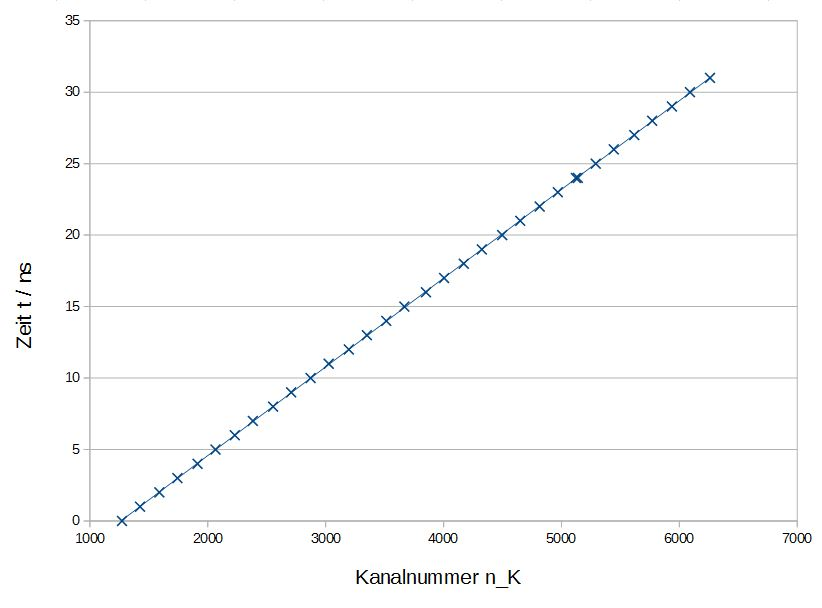
\includegraphics[width=0.7\columnwidth]{pics/Zeitkal}
			\caption{Messung zur Kalibrierung der Kanäle pro Zeit. Es ist die gemessene Zeit $t$ über die Kanalnummern $n_\textrm{K}$ aufgetragen. Die Grade durch die Messwerte ist eine lineare Regression.}
		\end{figure}
		\newpage
	\subsection{Bestimmung der Zerfallskonstanten}
		
		\begin{figure}[!h]
			\centering
			\label{abb:Messung1}
			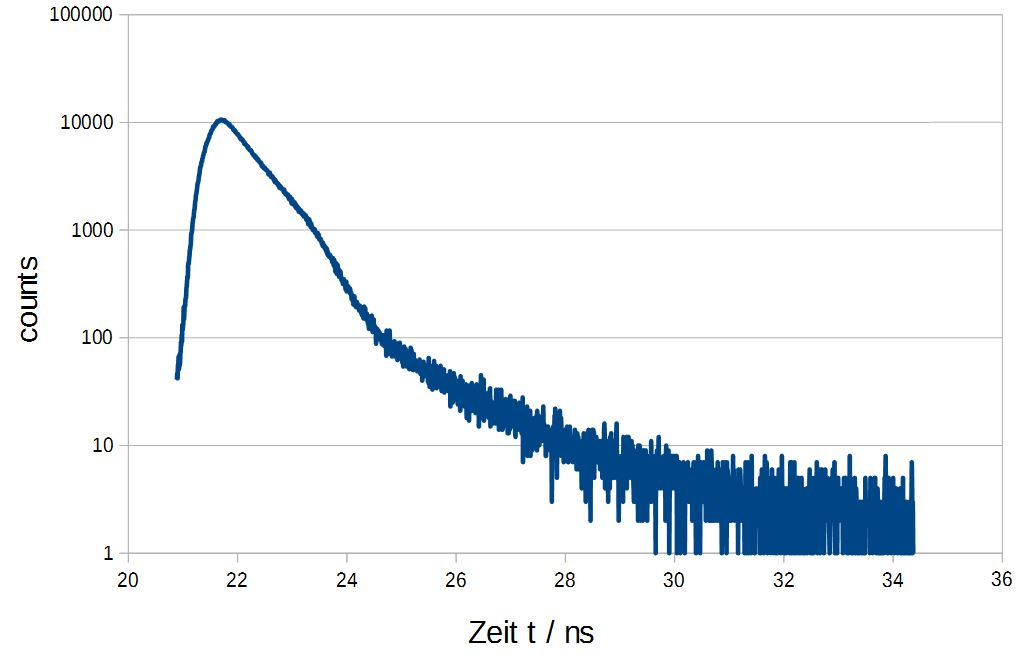
\includegraphics[width=0.7\columnwidth]{pics/Messung1}
			\caption{Logarithmisch skalierte Signalintensität der Koinzidenzmessung der bei der Rekombination entstandenen $\gamma$-Photonen. Die X-Achse ist nach \eqref{eq:Zeitkal} die Zeit abgetragen.}
		\end{figure}
		
		In der Abb.\ref{abb:Messung1} ist die logarithmisch skalierte Signalintensität der koinzident gemessenen $\gamma$-Photonen über die Vergangene Zeit aufgetragen.
		In dem Graphen sind drei verschiedene Zerfälle zu erkennen. Der erste liegt ungefähr im Zeitintervall von $21,8\,\mathrm{ns}$ bis $23,3\,\mathrm{ns}$ (Abschnitt 1), der zweite zwischen $23,3\,\mathrm{ns}$ und $24,5\,\mathrm{ns}$ (Abschnitt 2), und der letzte zwischen $24,5\,\mathrm{ns}$ und $28,0\,\mathrm{ns}$ (Abschnitt 3). Dabei ist anzumerken, dass der zweite Abschnitt den stärksten Abfall aufweist, während der dritte den schwächsten hat. Dies ist ungewöhnlich, da zu erwarten ist, das der erste Abschnitt den steilsten Abfall aufweisen sollte. 
		Für die Zerfälle wird jeweils ein exponentielles Zerfallsgesetz angenommen.
		\begin{equation}
			N_\mathrm{i}(t) = N_{\mathrm{i}0} \exp\left(-\lambda_\mathrm{i} t\right)
		\end{equation}
		Aus den Ansätzen lassen sich 3 Zerfallskonstanten $\lambda_\mathrm{i}$ bestimmen. Der Fehler dieser Konstanten ist gleich dem Fehler der Steigung der logarithmischen Darstellung
		\begin{equation}
			\ln\left(N_\mathrm{i}\right) = \ln\left(N_{\mathrm{i}0}\right) - \lambda_\mathrm{i}t
		\end{equation}
		berechnet. Die $\lambda_\mathrm{i}$ für die drei Intervalle sind
		\begin{align}
		\lambda_1 =& 1,425(4)\,\mathrm{ns}^{-1}, \nonumber \\
		\lambda_{2} =& 2,10(4)\,\mathrm{ns}^{-1},  \\
		\lambda_{3} =& 0,76(3)\,\mathrm{ns}^{-1}. \nonumber 
		\end{align}
		Die zu den Zerfallskonstanten gehörende Lebenszeit ist ihr Reziprokes
		\begin{equation}
			\tau_\mathrm{i} = \frac{1}{\lambda_\mathrm{i}}.
		\end{equation}
		Die resultierenden Lebenszeiten der beobachteten Zerfälle und deren Fehler ergibt sich zu
		\begin{align}
			\tau_{1} =& 0,702(2)\,\mathrm{ns} \nonumber \\
			\tau_{2} =& 0,476(9)\,\mathrm{ns} \\
			\tau_{3} =& 1,32(5)\,\mathrm{ns} \nonumber 
		\end{align}
	\subsection{Fazit}
		Die gemessenen Lebenszeiten $\tau_1$ und $\tau_2$ stimmen von der Größenordnung mit der des Parapositroniums überein ($0,142\,\mathrm{ns}$). Die verbleibenden Unterschiede können dadurch erklärt werden, da in der Messung nicht die Zeit berücksichtigt wird, welche das Positron braucht um genügend Energie abzugeben, um eine Bindung mit einem Elektron einzugehen. Die Lebenszeit des Orthopositroniums liegt jedoch mehrere Größenordnungen über den gemessenen Zeiten ($142\,\mathrm{ns}$) und kann keiner Lebensdauer zugeordnet werden.\\
		
		
		Zusammenfassend kann gesagt werden, dass der Versuch einen Einblick in den Aufbau von anspruchsvollerer Messelektronik gegeben hat und vor allem das Prinzip der Koinzidensmessung verdeutlicht hat, aber die eigentliche Messung leider nicht zu Ende ausgewertet werden konnte. 
		\newpage

\section{Anhang}
\subsection{Quellen}
\begin{enumerate}
	\item Praktikumsanleitung zum Fortgeschrittenen Praktikum "Positronen Koinzidensmessungen", 21.10.2015, EMA-Universität Greifswald
	\item Wikipedia Artikel zu Positronen https://en.wikipedia.org/wiki/Positronium 23.10.2015
	\item Christian Augsten. Asymmetrische Fluß Feld-Fluß Fraktionierung in Verbindung mit
	Mehrwinkellichtstreudetektion: Eine neue bedeutende Methode der Pharmazeutischen
	Analytik zur Charakterisierung von Makromolekülen und Nanopartikeln. Online-
	Dokument, Dissertation, Universitätsbibliothek Halle, pages 4–17, 2008.
	\item Programm zur linearen Regression "REGRESSION.exe", B. Pompe 07.11.2002
\end{enumerate}
\subsection{Weitere Graphen}

\begin{figure}[!h]
	\centering
	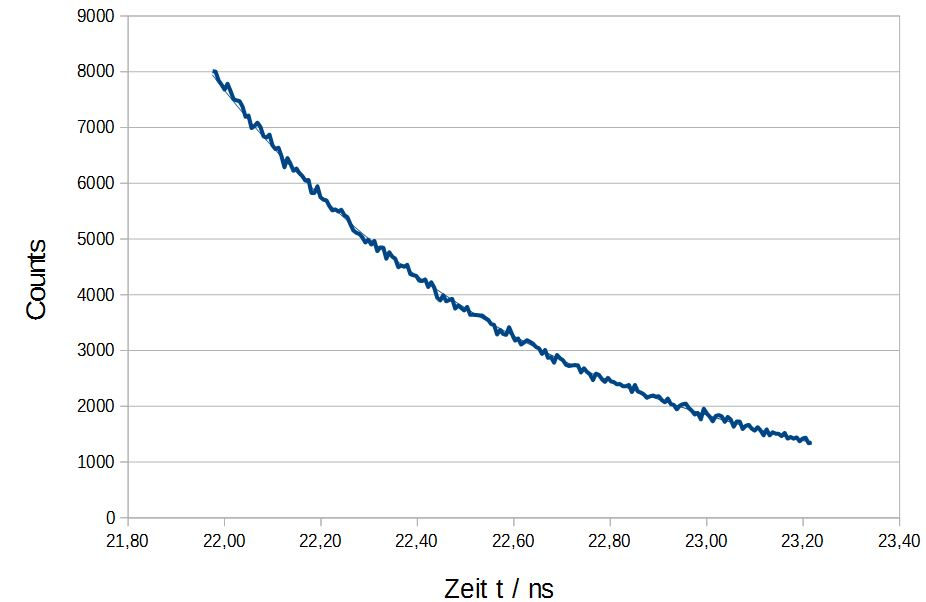
\includegraphics[width=0.7\columnwidth]{pics/Messung2a}
	\caption{Ausschnitt 1 aus der zeitaufgelösten Messung der Positronenlebensdauer. Die Kurve im Graphen ist ein exponentieller Fit.}
\end{figure}
\begin{figure}[!h]
	\centering
	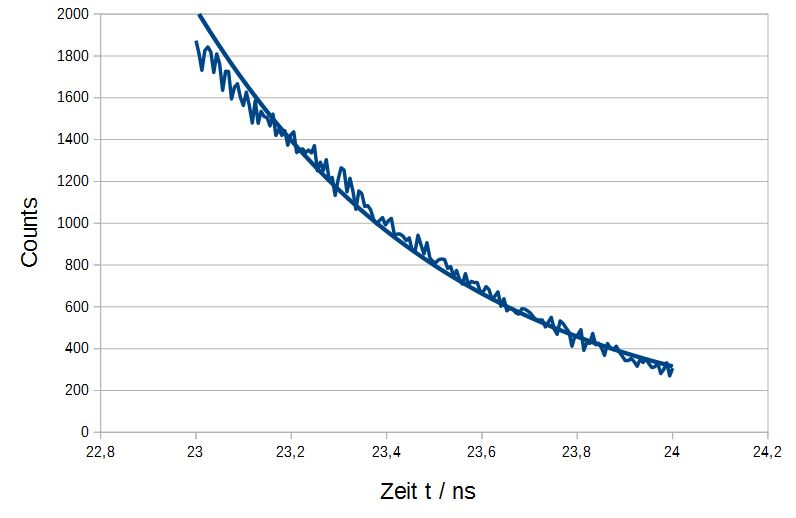
\includegraphics[width=0.7\columnwidth]{pics/Messung2b}
	\caption{Ausschnitt 2 aus der zeitaufgelösten Messung der Positronenlebensdauer. Die Kurve im Graphen ist ein exponentieller Fit.}
\end{figure}
\begin{figure}[!h]
	\centering
	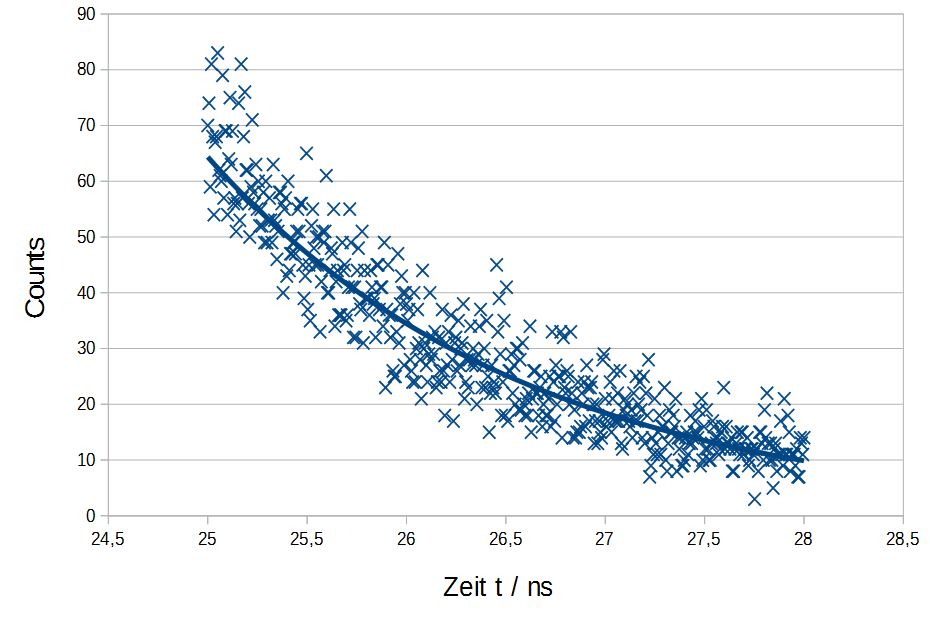
\includegraphics[width=0.7\columnwidth]{pics/Messung2c}
	\caption{Ausschnitt 3 aus der zeitaufgelösten Messung der Positronenlebensdauer. Die Kurve im Graphen ist ein exponentieller Fit.}
\end{figure}

\end{document}